\chapter{ZigBee - WSN Case Study}

\begin{figure}[htbp]
   \centering
   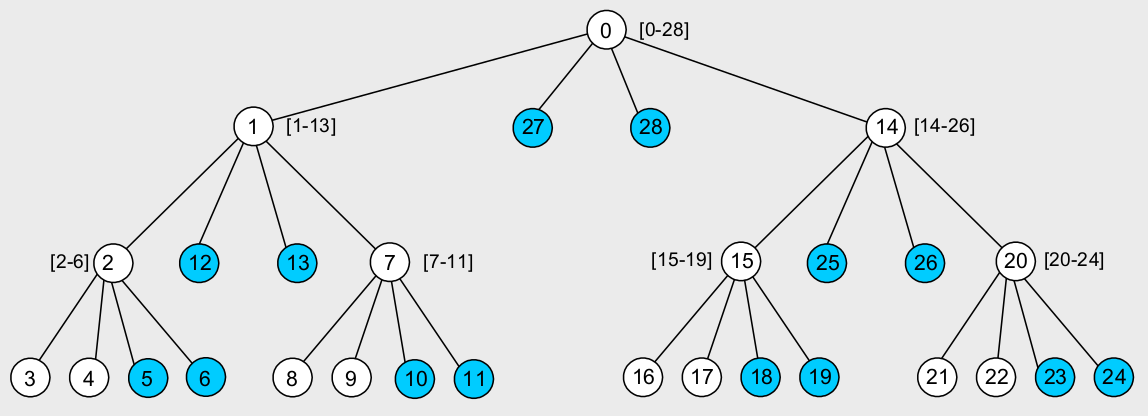
\includegraphics{images/zigbee_tree.png}\\
   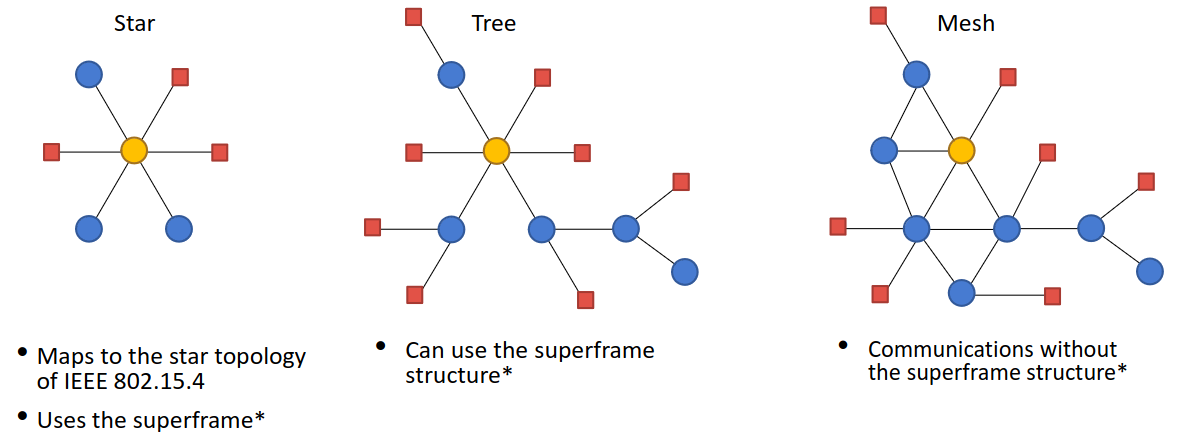
\includegraphics{images/zigbee_networktopologies.png}
   \caption{ZigBee tree topology example with assigned address ranges. Comparison between star/tree/mesh topologies.}
   \label{fig:zigbee_tree}
\end{figure}

The tree topology is used to assign the short network addresses, the ZigBee coordinator is statically configured with:
\begin{itemize}
   \item The maximum number of routers (Rm) each router may have as
   children
   \item The maximum number of end-devices (Dm) that each router may
   have as children
   \item The maximum depth of the tree (Lm).
\end{itemize}
Each router is assigned with a range of addresses
\begin{itemize}
   \item To assign addresses to its children
   \item Computed based on Rm, Dm, and Lm.
\end{itemize}

Devices join as high up the tree as possible, minimizing the number of hops.
Although the addresses are assigned according to a tree structure the actual topology can be a mesh.

\section{Routing}
\textbf{Tree routing} is used to route packets between devices that are directly connected.
It exploits beaconing to maintain the tree structure.

\textbf{Mesh routing} routing is used to route packets between devices that are not directly connected.
When no entry for the destination is  in the routing table, \textit{route discovery} is performed.
Mesh does \textit{not} allow beaconing.

Tree and mesh topologies may coexist in the same network.